\quiz{2022-119}{https://net-sci-questions.blogspot.com/2022/05/2022-099.htmll}

Starting from the node indicated as `start', use DFS and label the nodes with their ending times. Which of the alternatives below corresponds to a possible answer?

\begin{figure}[H]
    \centering
    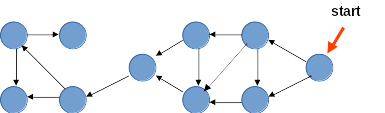
\includegraphics{images/119-0.png}
\end{figure}

Tip: the reverse order of finishing DFS times in a directed acyclic graph is a topological order.

\begin{enumerate}[label={\Alph*.}]

\raggedcolumns\begin{multicols}{2}
    \item 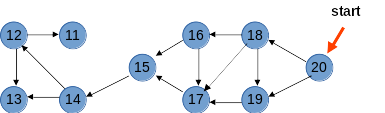
\includegraphics[width=0.45\textwidth]{images/119-A.png}

    \item 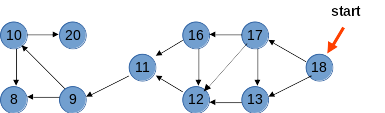
\includegraphics[width=0.45\textwidth]{images/119-B.png}
\end{multicols}

\raggedcolumns\begin{multicols}{2}
    \item 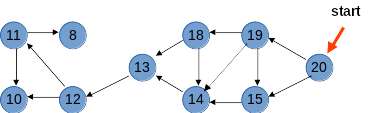
\includegraphics[width=0.45\textwidth]{images/119-C.png}

    \item 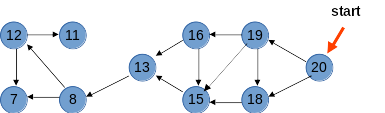
\includegraphics[width=0.45\textwidth]{images/119-D.png}
\end{multicols}

    \item None of the above
\end{enumerate}

Original ideia by: Filipe Maciel Roberto
